\nonstopmode
\documentclass{beamer}
\usepackage{listings}
\usepackage{fancyvrb}

\usepackage{pgf}
\usepackage[english]{babel}
\usepackage[latin1]{inputenc}
\usepackage{times}
\mode<article>
{
  \usepackage{times}
  \usepackage{mathptmx}
  \usepackage[left=1.5cm,right=6cm,top=1.5cm,bottom=3cm]{geometry}
}

\usepackage{hyperref}
\usepackage[T1]{fontenc}
\usepackage{tikz}
\usepackage{colortbl}
%\usepackage{yfonts}
%\usepackage{colortbl}
%\usepackage{translator} % comment this, if not available


% Common settings for all lectures in this course

\def\lecturename{A Proposal for BEAST 2.0}

\title{\insertlecture}

\author{Till Tantau}

\institute
{
  Institut für Theoretische Informatik\\
  Universität zu Lübeck
}

\subject{Vorlesung \lecturename}




% Beamer version theme settings

\useoutertheme[height=0pt,width=2cm,right]{sidebar}
\usecolortheme{rose,sidebartab}
\useinnertheme{circles}
\usefonttheme[only large]{structurebold}

\setbeamercolor{sidebar right}{bg=black!15}
\setbeamercolor{structure}{fg=blue}
\setbeamercolor{author}{parent=structure}

\setbeamerfont{title}{series=\normalfont,size=\LARGE}
\setbeamerfont{title in sidebar}{series=\bfseries}
\setbeamerfont{author in sidebar}{series=\bfseries}
\setbeamerfont*{item}{series=}
\setbeamerfont{frametitle}{size=}
\setbeamerfont{block title}{size=\small}
\setbeamerfont{subtitle}{size=\normalsize,series=\normalfont}

\setbeamertemplate{navigation symbols}{}
\setbeamertemplate{bibliography item}[book]
\setbeamertemplate{sidebar right}
{
  {\usebeamerfont{title in sidebar}%
    \vskip1.5em%
    \hskip3pt%
    \usebeamercolor[fg]{title in sidebar}%
    \insertshorttitle[width=2cm,center,respectlinebreaks]\par%
    \vskip1.25em%
  }%
  {%
    \hskip3pt%
    \usebeamercolor[fg]{author in sidebar}%
    \usebeamerfont{author in sidebar}%
    \insertshortauthor[width=2cm,center,respectlinebreaks]\par%
    \vskip1.25em%
  }%
  \hbox to2cm{\hss\insertlogo\hss}
  \vskip1.25em%
  \insertverticalnavigation{2cm}%
  \vfill
  \hbox to 2cm{\hfill\usebeamerfont{subsection in
      sidebar}\strut\usebeamercolor[fg]{subsection in
      sidebar}%\insertshortlecture.
      \insertframenumber\hskip5pt}%
  \vskip3pt%
}%

\setbeamertemplate{title page}
{
  \vbox{}
  \vskip1em
 % {\huge \insertshortlecture\par}
  {\usebeamercolor[fg]{title}\usebeamerfont{title}\inserttitle\par}%
  \ifx\insertsubtitle\@empty%
  \else%
    \vskip0.25em%
    {\usebeamerfont{subtitle}\usebeamercolor[fg]{subtitle}\insertsubtitle\par}%
  \fi%     
  \vskip1em\par
  %Vorlesung \emph{\lecturename}\ vom \insertdate\par
  \vskip0pt plus1filll
  \leftskip=0pt plus1fill\insertauthor\par
  \insertinstitute\vskip1em
}

\logo{
\includegraphics[width=1cm]{auckland.png}}



% Article version layout settings

\mode<article>

\makeatletter
\def\@listI{\leftmargin\leftmargini
  \parsep 0pt
  \topsep 5\p@   \@plus3\p@ \@minus5\p@
  \itemsep0pt}
\let\@listi=\@listI


\setbeamertemplate{frametitle}{\paragraph*{\insertframetitle\
    \ \small\insertframesubtitle}\ \par
}
\setbeamertemplate{frame end}{%
  \marginpar{\scriptsize\hbox to 1cm{\sffamily%
      \hfill\strut%\insertshortlecture.
    \insertframenumber}\hrule height .2pt}}
\setlength{\marginparwidth}{1cm}
\setlength{\marginparsep}{4.5cm}




\let\origstartsection=\@startsection
\def\@startsection#1#2#3#4#5#6{%
  \origstartsection{#1}{#2}{#3}{#4}{#5}{#6\normalfont\sffamily\color{blue!50!black}\selectfont}}

\makeatother

\mode
<all>




% Typesetting Listings

\usepackage{listings}
\lstset{language=Java}

\alt<presentation>
{\lstset{%
  basicstyle=\footnotesize\ttfamily,
  commentstyle=\slshape\color{blue!50!black},
  keywordstyle=\bfseries\color{blue!50!black},
  identifierstyle=\color{blue},
  stringstyle=\color{orange},
  escapechar=\#,
  emphstyle=\color{red}}
}
{
  \lstset{%
    basicstyle=\ttfamily,
    keywordstyle=\bfseries,
    commentstyle=\itshape,
    escapechar=\#,
    emphstyle=\bfseries\color{red}
  }
}



% Common theorem-like environments

\theoremstyle{definition}
\newtheorem{exercise}[theorem]{\translate{Exercise}}




% New useful definitions:

\newbox\mytempbox
\newdimen\mytempdimen

\newcommand\includegraphicscopyright[3][]{%
  \leavevmode\vbox{\vskip3pt\raggedright\setbox\mytempbox=\hbox{\includegraphics[#1]{#2}}%
    \mytempdimen=\wd\mytempbox\box\mytempbox\par\vskip1pt%
    \fontsize{3}{3.5}\selectfont{\color{black!25}{\vbox{\hsize=\mytempdimen#3}}}\vskip3pt%
}}

\newenvironment{colortabular}[1]{\medskip\rowcolors[]{1}{blue!20}{blue!10}\tabular{#1}\rowcolor{blue!40}}{\endtabular\medskip}

\def\equad{\leavevmode\hbox{}\quad}

\newenvironment{bluecolortabular}[1]
{\medskip\rowcolors[]{1}{blue!50!black!20}{blue!50!black!10}%
  \tabular{#1}\rowcolor{blue!50!black!40}}%
{\endtabular\medskip}


%\mode<presentation>
%{
%  \usetheme{PaloAlto}
%  \usetheme{Bergen}
  %\usetheme{Berkeley}
  %\setbeamercovered{transparent}
%}


\usepackage[english]{babel}
\usepackage[latin1]{inputenc}
\usepackage{times}
\usepackage[T1]{fontenc}

\title[Beast 2.0]
{A Proposal for Beast 2.0}

%\subtitle{}

\author[Bouckaert] 
{Remco R. Bouckaert\\\url{remco@cs.{auckland|waikato}.ac.nz}}

\institute[University of Auckland|Waikato]
{Department of Computer Science\\
  University of Auckland \& University of Waikato
}
\date[] % (optional)
{}

\subject{A Proposal for Beast 2.0}


% If you wish to uncover everything in a step-wise fashion, uncomment
% the following command: 

%\beamerdefaultoverlayspecification{<+->}


\begin{document}

\begin{frame}
  \titlepage
\end{frame}


\section{Vision}
\begin{frame}{Vision}
To provide tools for computational science that are
\begin{itemize}
\item
{\em easy to use}, that is, well documented, have intuitive user interfaces with small learning curve.
\item
{\em open access}, that is, open source, open xml format, facilitating reproducability of results, runs
on many platforms.
\item
{\em easy to extend}, by having extensibility in design.
\end{itemize}
\vskip1cm
{\bf\large\color{blue} Scope}
\vskip0.5cm
Efficient testing of probabilistic hypotheses for sequence data analysis involving tree models.

\end{frame}

\begin{frame}{Vision}
To provide tools for computational science that are
\begin{itemize}
\item
{\em easy to use}, that is, {\color{red} well documented}, have intuitive user interfaces with small learning curve.
\item
{\em open access}, that is, open source, open xml format, facilitating reproducability of results, runs
on many platforms.
\item
{\em {\color{red} easy to extend}}, by having extensibility in design.
\end{itemize}
\vskip1cm
{\bf\large\color{blue} Scope}
\vskip0.5cm
{\color{orange} Efficient} testing of probabilistic hypotheses for sequence data analysis involving tree models.

\end{frame}


\section{Basic design}

\begin{frame}{Core}
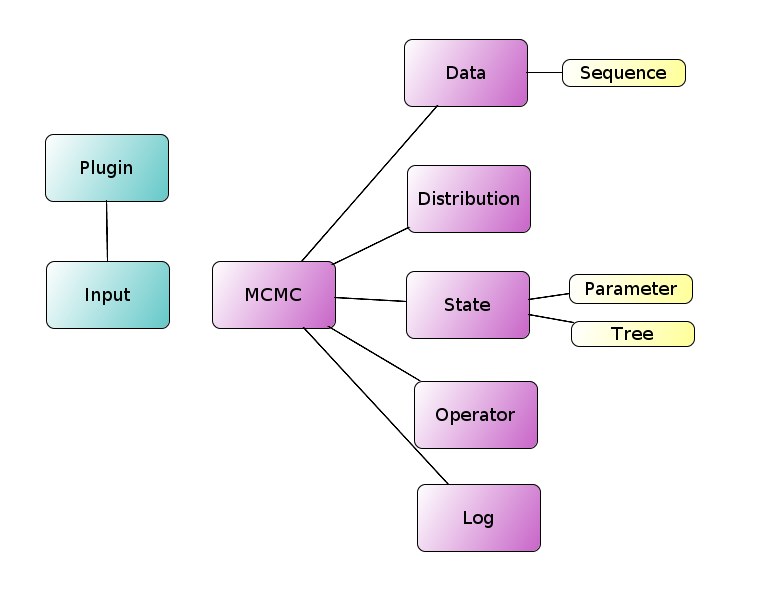
\includegraphics[width=\textwidth]{BEAST.png}
\end{frame}

\begin{frame}[containsverbatim]
{\Large Phylosophy}

Everything is a plug-in
\vskip0.5cm
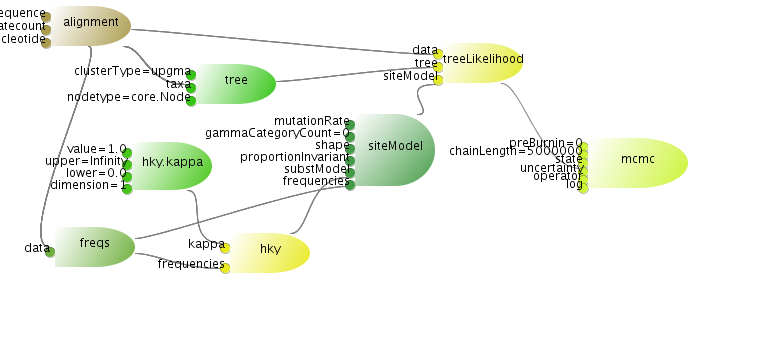
\includegraphics[width=\textwidth]{hkymodel.png}

Plug-ins provide...
\begin{itemize}
\item connection with with other plug-ins/values through 'inputs'
\item validation
\item documentation
\item 'XML parsing'
\end{itemize}
\end{frame}

\begin{frame}[containsverbatim]
{\Large Plugin class}

\begin{lstlisting}[language=java]
@Description("Description goes here")
public class Plugin {
    public void initAndValidate(State state)

    public String getCitations()

    public String getID()
    public void setID(String sID)

    public void store(int nSample)
    public void restore(int nSample)
} // class Plugin
\end{lstlisting}

\end{frame}
\begin{frame}[containsverbatim]
{\large HKY Plugin}

{
%\lstset{basicstyle=\small}
\tiny
\begin{lstlisting}[language=java]
@Description("HKY85 (Hasegawa, Kishino & Yano, 1985) substitution model of nucleotide evolution.")
public class HKY extends 'Plugin' {
    public Input<Frequencies> m_freqs = new Input<Frequencies>("frequencies", "frequencies nucleotide letters");
    public Input<Parameter> m_kappa = new Input<Parameter>("kappa", "kappa parameter in HKY model", Validate.REQUIRED);

    @Override public void initAndValidate(State state) throws Exception {
        initialiseEigen();        
    }

    public void getTransitionProbabilities(double distance, double[] matrix, State state) {
        ...
    }
    @Override public void store(int nSample) {}
    @Override public void restore(int nSample) {
        updateMatrix = true;
        updateIntermediates = true;
    }
    @Override public String getCitation() {
        return "Hasegawa, M., Kishino, H and Yano, T. 1985. Dating the human-ape splitting by a molecular clock of mitochondrial DNA. Journal of Molecular Evolution 22:160-174.";
    }
} // class HKY
\end{lstlisting}
}
\end{frame}

\begin{frame}[containsverbatim]
{\Large Inputs}
\pgfputat{\pgfxy(5,-1)}{\pgfbox[left,base]{\pgfimage[width=5cm]{hkymodel.png}}}
Simple primitives

\begin{lstlisting}[language=java]
public Input<Boolean> m_pScaleAll = 
    new Input<Boolean>("scaleAll", 
        "if true, all elements of a parameter (not tree) are scaled, otherwise one is randomly selected",
        new Boolean(false));
\end{lstlisting}

Other plugins

\begin{lstlisting}[language=java]
public Input<Frequencies> m_freqs = 
    new Input<Frequencies>("frequencies", 
        "frequencies nucleotide letters");
\end{lstlisting}

Multiple inputs

\begin{lstlisting}[language=java]
public Input<List<Parameter>> m_pParameters = 
    new Input<List<Parameter>>("parameter", 
        "parameter, part of the state",
        new ArrayList<Parameter>());
\end{lstlisting}
\end{frame}

\begin{frame}[containsverbatim]
{\Large Input validation}

Default: OPTIONAL (see previous slide)
\vskip0.2cm
If input is REQUIRED:

\begin{lstlisting}[language=java]
public Input<Parameter> m_kappa = 
    new Input<Parameter>("kappa", 
        "kappa parameter in HKY model",
        Validate.REQUIRED);
\end{lstlisting}

\begin{lstlisting}[language=java]
public Input<List<Operator>> m_operators = 
    new Input<List<Operator>>("operator",
        "operator for generating proposals in MCMC state space",
        new ArrayList<Operator>(), Validate.REQUIRED);
\end{lstlisting}

If input is XOR:

\begin{lstlisting}[language=java]
public Input<Tree> m_pTree = 
    new Input<Tree>("tree", 
        "if specified, all tree branch length are scaled");
public Input<Parameter> m_pParameter = 
    new Input<Parameter>("parameter", 
        "if specified, this parameter is scaled"
        , Validate.XOR, m_pTree);
\end{lstlisting}

\end{frame}


\begin{frame}[containsverbatim]
{\Large State}
\begin{itemize}
\item State is explicit in XML \& as object (unlike Beast 1)
\item Contains parameters and trees
\item Operators work on the state
\begin{lstlisting}[language=java]
public double proposal(State state) throws Exception {...}
\end{lstlisting}
\item Uncertainty calculated given state
\begin{lstlisting}[language=java]
public double calculateLogP(State state) throws Exception {...}
\end{lstlisting}
\item State can be interrogated on value of parameters/trees
\begin{lstlisting}[language=java]
state.getParameter(/**Parameter**/ p)
state.getTree(/**Tree**/ t)
\end{lstlisting}
\end{itemize}
\end{frame}

\begin{frame}[containsverbatim]
{\Large Store/Restore}

BEAST 1: push model
\begin{itemize}
\item Model
\item Event handling
\item Framework and plug-ins responsible
\item Elegant, undocumented, requires lots of Panadol
\end{itemize}

BEAST 2: pull model
\begin{itemize}
\item store/restore 
\item sample number provided to prevent multiple (re)stores
\item MCMC only tells its 'uncertainties' to store/restore, plug-ins responsible
\end{itemize}
\end{frame}



\section{XML}

\begin{frame}{XML}
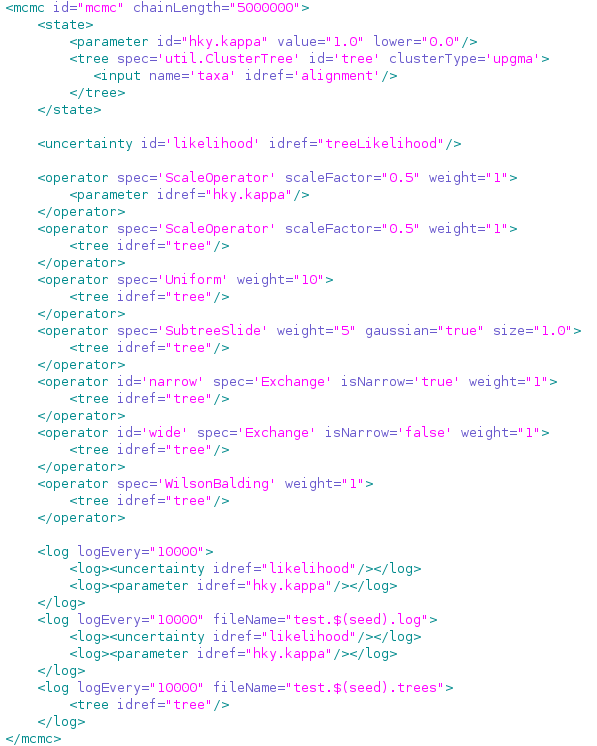
\includegraphics[width=1.25\textwidth]{xml3.png}
\end{frame}
\begin{frame}[containsverbatim]
XML parsing/writing provided by the framework
{\Large XML}
Reserved elements
\pgfputat{\pgfxy(1.5,-4)}{\pgfbox[left,base]{\pgfimage[width=5cm]{BEAST.png}}}
\begin{Verbatim}[commandchars=\\\{\}]
\textcolor{blue}{\bf <mcmc}\textcolor{blue}{\bf >}
\textcolor{blue}{\bf <uncertainty}\textcolor{blue}{\bf >}
\textcolor{blue}{\bf <operator}\textcolor{blue}{\bf >}
\textcolor{blue}{\bf <log}\textcolor{blue}{\bf >}
\textcolor{blue}{\bf <data}\textcolor{blue}{\bf >}
\textcolor{blue}{\bf <sequence}\textcolor{blue}{\bf >}
\textcolor{blue}{\bf <state}\textcolor{blue}{\bf >}
\textcolor{blue}{\bf <parameter}\textcolor{blue}{\bf >}
\textcolor{blue}{\bf <tree}\textcolor{blue}{\bf >}

\textcolor{blue}{\bf <beast} \textcolor{purple}{version=}\textcolor{black}{'2.0'} \textcolor{purple}{namespace=}\textcolor{black}{'x.y.z:'}\textcolor{blue}{\bf >}
\textcolor{blue}{\bf <map} \textcolor{purple}{name=}\textcolor{black}{'elementName'}\textcolor{blue}{\bf >}x.y.z.Class\textcolor{blue}{\bf </map>}
\end{Verbatim}
\end{frame}

\begin{frame}{XML}
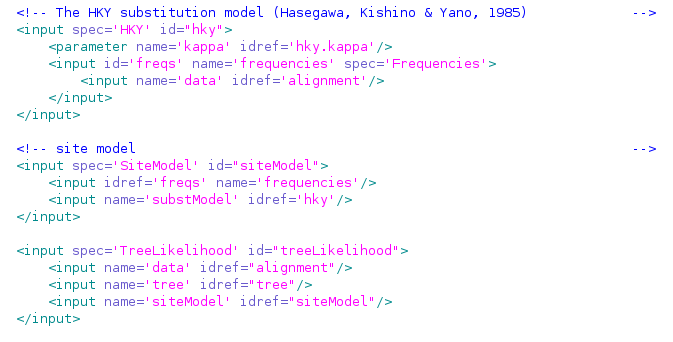
\includegraphics[width=1.25\textwidth]{xml1.png}
\end{frame}
\begin{frame}{XML}
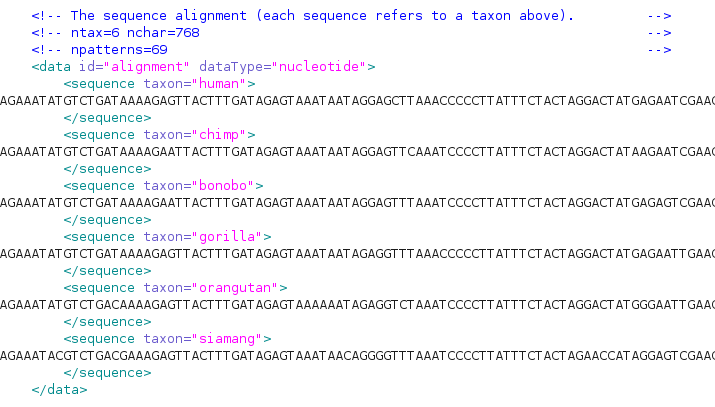
\includegraphics[width=1.25\textwidth]{xml2.png}
\end{frame}


\begin{frame}[containsverbatim]
{\Large XML}
Reserved attributes:
\begin{Verbatim}[commandchars=\\\{\}]
\textcolor{blue}{\bf  <input} \textcolor{purple}{id=}\textcolor{black}{'myId'} 
     \textcolor{purple}{idref=}\textcolor{black}{'otherId'} 
     \textcolor{purple}{name=}\textcolor{black}{'inputName'} 
     \textcolor{purple}{spec=}\textcolor{black}{'x.y.z.MyClass'}\textcolor{blue}{\bf  />}
\end{Verbatim}
\vskip0.5cm
Resolving plug-in class:
\begin{itemize}
\item specified in spec attribute
\item if not, get from element2class map
\item if not, use element name (and hope it shows up in the namespace somewhere).
\end{itemize}
\end{frame}


\begin{frame}[containsverbatim]
{\Large XML}
Resolving input name:
\begin{itemize}
\item specified in name attribute
\begin{lstlisting}[language=java]
    <input name="xyz" >
\end{lstlisting}
\item if not, use (non-reserved) attribute name
\begin{lstlisting}[language=java]
    <input xyz="3" >
\end{lstlisting}
\item if not, use element name
\begin{lstlisting}[language=java]
    <xyz value="3" >
\end{lstlisting}
\item if input, use 'value' when there is text content, but no element content
\begin{lstlisting}[language=java]
    <input>3</input>
\end{lstlisting}
\end{itemize}
\end{frame}


\begin{frame}[containsverbatim]
{\Large XML}
Resolving input value:
\begin{itemize}
\item if idref is specified, use the referred object
\begin{lstlisting}[language=java]
    <input idref="other" >
\end{lstlisting}
\item specified in value attribute
\begin{lstlisting}[language=java]
    <xyz value="3" >
\end{lstlisting}
\item if not, use value of (non-reserved) attribute
\begin{lstlisting}[language=java]
    <input xyz="3" >
\end{lstlisting}
\item if not, use text content when there is text content, but no element content
\begin{lstlisting}[language=java]
    <input>3</input>
\end{lstlisting}
\end{itemize}
\end{frame}


\begin{frame}[containsverbatim]
{\Large XML}
Parsing rules:
Processing non reserved attributes
\begin{Verbatim}[commandchars=\\\{\}]
\textcolor{blue}{\bf  <input} \textcolor{purple}{otherAttribute=}\textcolor{black}{"xyz"}\textcolor{blue}{\bf  />}
\end{Verbatim}
equals
\begin{Verbatim}[commandchars=\\\{\}]
\textcolor{blue}{\bf  <input}\textcolor{blue}{\bf  >}
  \textcolor{blue}{\bf  <input} \textcolor{purple}{name=}\textcolor{black}{'otherAttribute'} \textcolor{purple}{value=}\textcolor{black}{'xyz'}\textcolor{blue}{\bf  />}
\textcolor{blue}{\bf  </input>}
\end{Verbatim}

Processing non reserved element names
\begin{Verbatim}[commandchars=\\\{\}]
\textcolor{blue}{\bf  <myElement}\textcolor{blue}{\bf  />}
\end{Verbatim}
==
\begin{Verbatim}[commandchars=\\\{\}]
\textcolor{blue}{\bf  <input} \textcolor{purple}{spec=}\textcolor{black}{'myElement'} \textcolor{purple}{name=}\textcolor{black}{'myElement'}\textcolor{blue}{\bf  />}
\end{Verbatim}
unless 'spec' is a specified attribute, then that overrides, likewise for 'name' 
%\end{frame}


%\begin{frame}[containsverbatim]
%{\Large XML}
Processing of text content (only when there are no enclosing elements)
\begin{Verbatim}[commandchars=\\\{\}]
\textcolor{blue}{\bf  <input} \textcolor{purple}{name=}\textcolor{black}{'data'}\textcolor{blue}{\bf  >}xyz\textcolor{blue}{\bf  </input>}
\end{Verbatim}
==
\begin{Verbatim}[commandchars=\\\{\}]
\textcolor{blue}{\bf  <input} \textcolor{purple}{name=}\textcolor{black}{'data'} \textcolor{purple}{value=}\textcolor{black}{'xyz'/}\textcolor{blue}{\bf  >}
\end{Verbatim}
\end{frame}


\section{Applications}


\begin{frame}{Model builder}
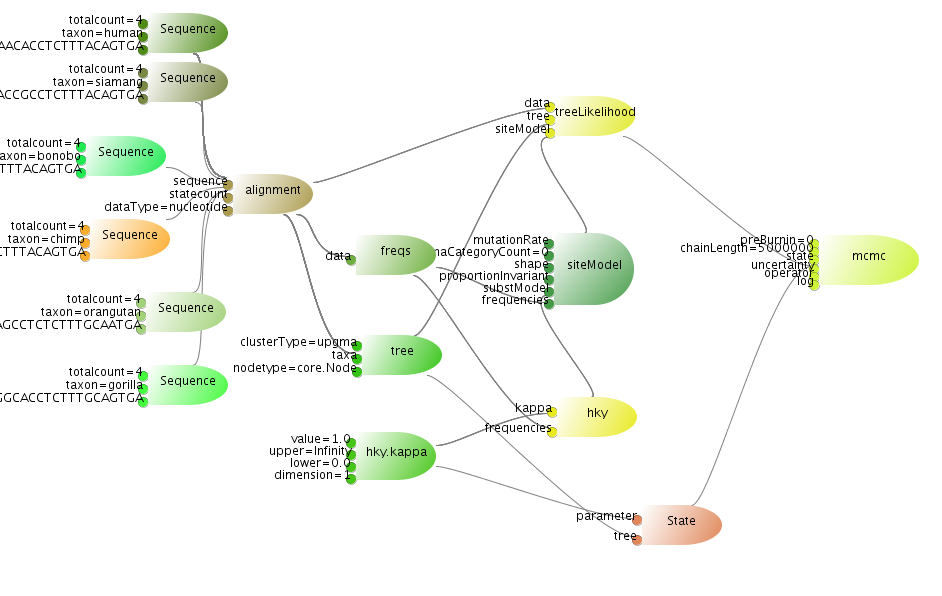
\includegraphics[width=\textwidth]{hkymodel2.png}
\end{frame}


\begin{frame}{Documentation}
XML documentation provided through

\begin{itemize}
\item @Description annotation on plug in
\item Tooltip text on inputs
\item getCitation method
\item Input validation rules
\end{itemize}

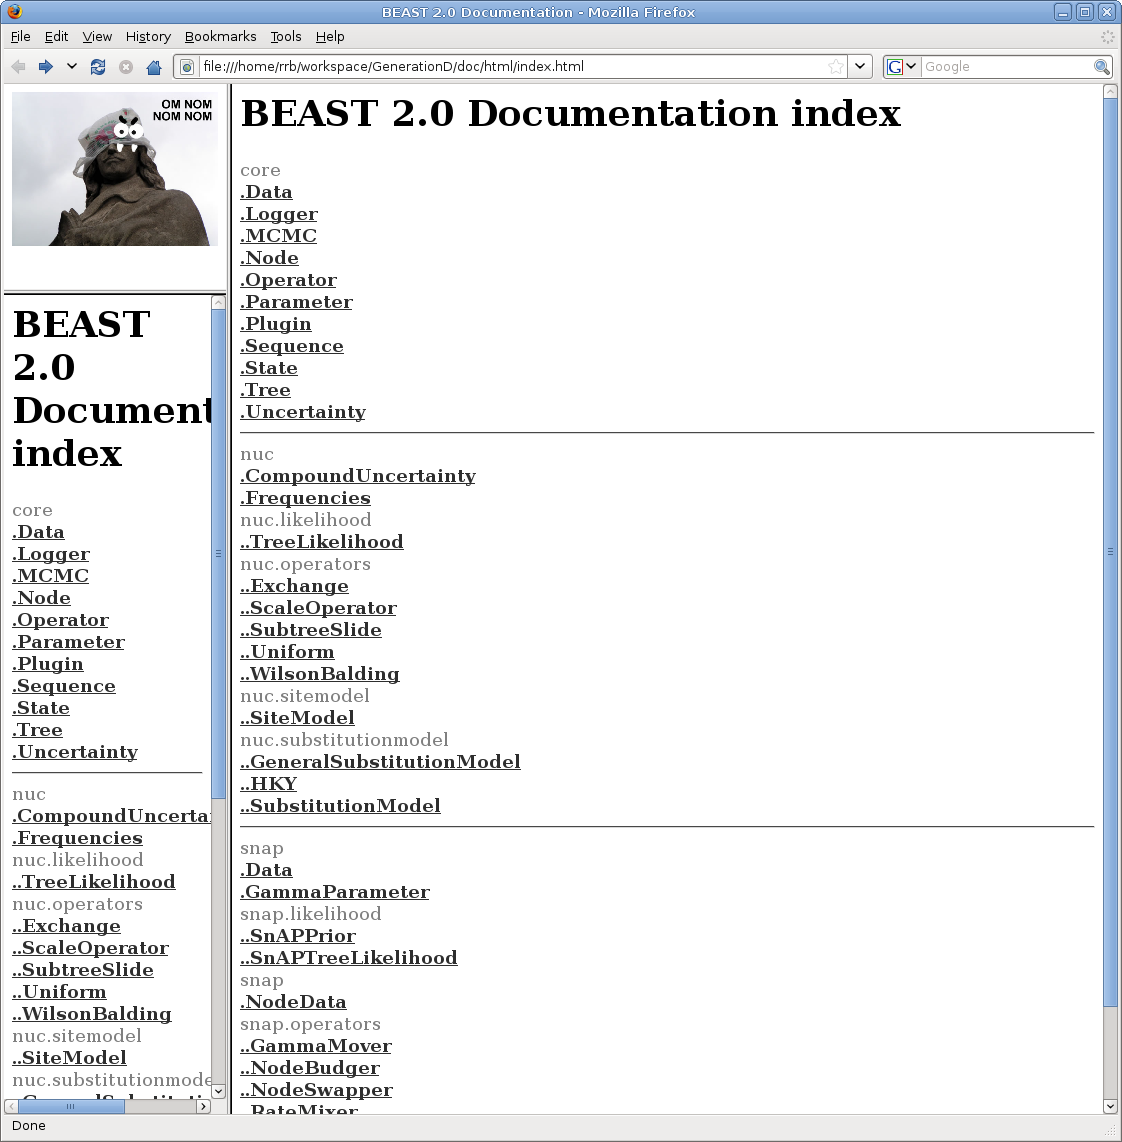
\includegraphics[width=\textwidth]{beastdoc0.png}

\end{frame}

\begin{frame}{Documentation}
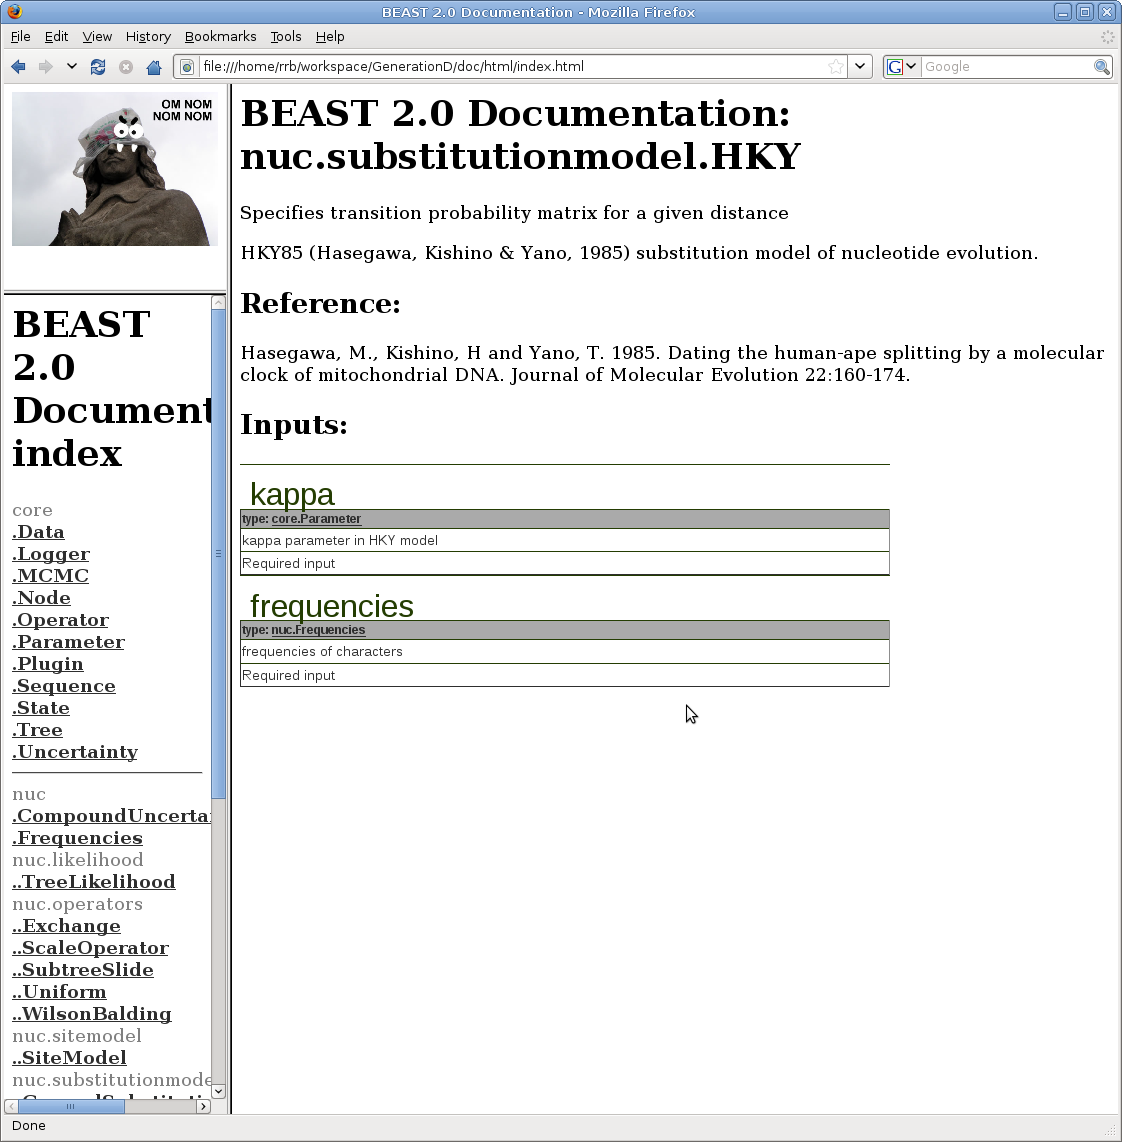
\includegraphics[width=\textwidth]{beastdoc1.png}
\end{frame}
\begin{frame}{Documentation}
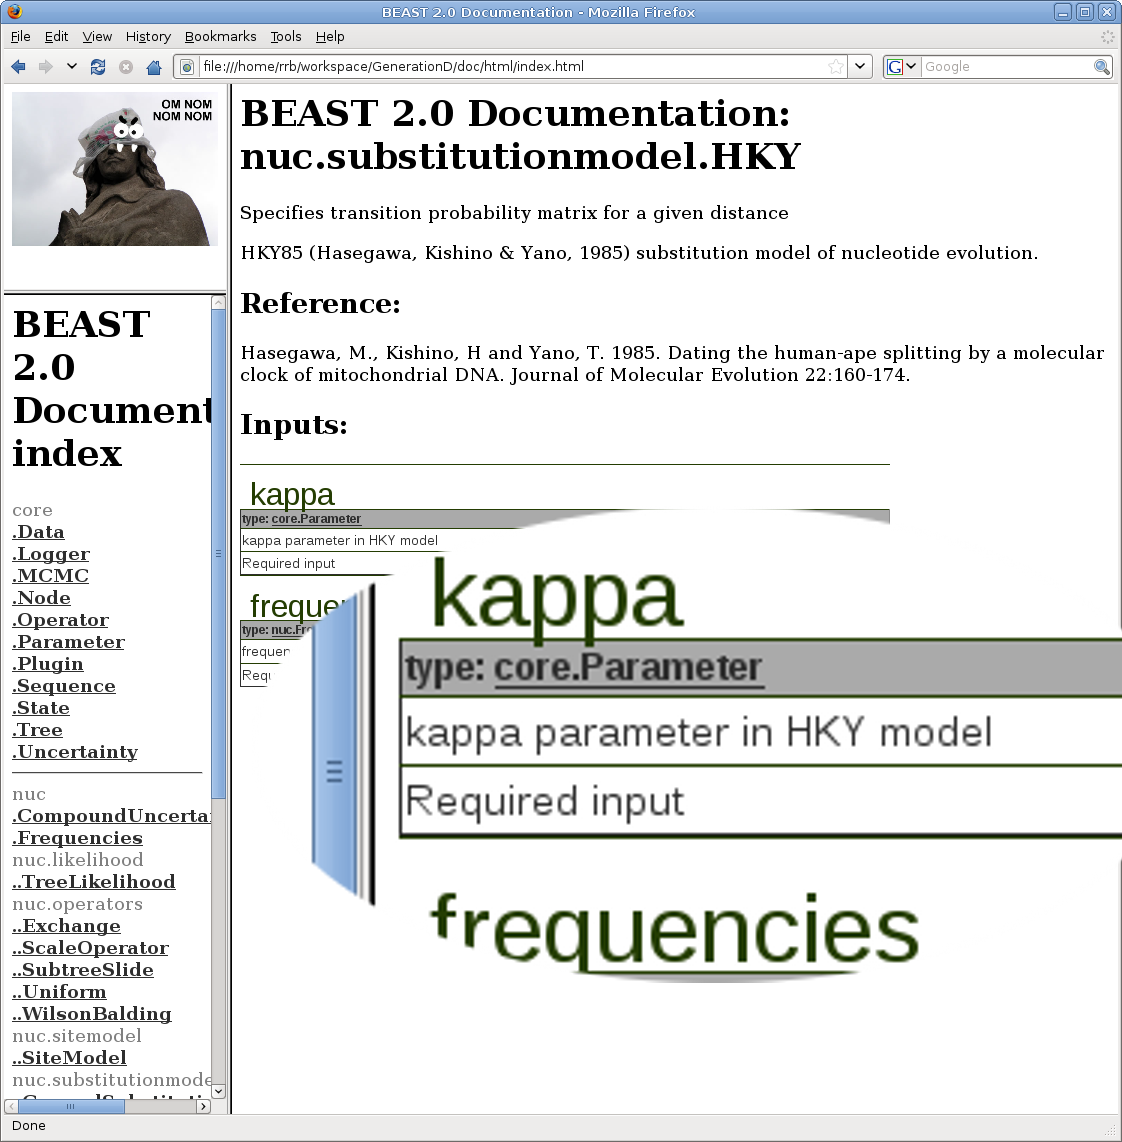
\includegraphics[width=\textwidth]{beastdoc2.png}
\end{frame}
\begin{frame}{Documentation}
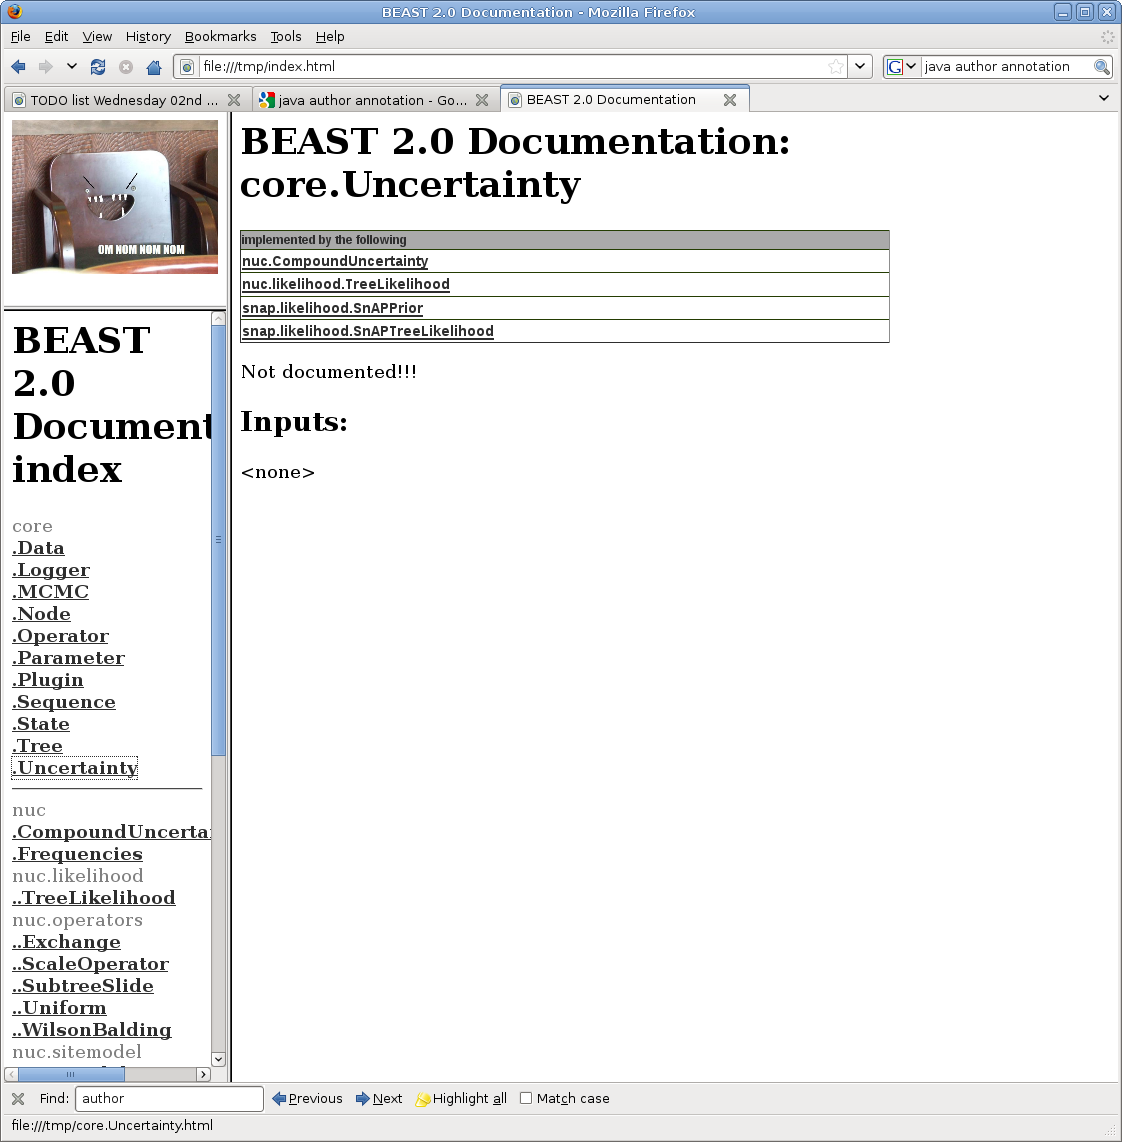
\includegraphics[width=\textwidth]{beastdoc4.png}
\end{frame}


\begin{frame}[containsverbatim]
{\Large BEAST 2.0}

\begin{lstlisting}[language=java]
~> java -cp bin app.BeastMCMC

Usage: BeastMCMC [options] <Beast.xml>
where <Beast.xml> the name of a file specifying a Beast run
and the following options are allowed:
-seed <int> : sets random number seed (default 127)
-threads <int> : sets number of threads (default 1)
\end{lstlisting}

\end{frame}

\begin{frame}[containsverbatim]
{\Large BEAST 2.0}
HKY + nucleotide data, 'random' initial tree

2000 samples in debug mode, scaling if required, auto optimise on, same logging, operators. etc.

testMCMC.xml -- great apes

\begin{verbatim}
6 taxa 
768 sites
69 patterns
10M samples  single thread
        Beast 1.6/java  Beast1.6/native Beast 2.0
real    3m55.056s       3m38.670s       2m31.794s
user    3m54.839s       3m38.670s       2m32.162s
sys     0m0.392s        0m0.428s        0m0.476s
\end{verbatim}
\end{frame}


\begin{frame}[containsverbatim]
{\Large BEAST 2.0}
testMCMC.xml -- 

\begin{verbatim}
46 taxa
1363 sites
199 patterns
500K samples 

Beast1.6/native core
real   1m56.097s
user   1m58.683s
sys    0m0.332s

Beast 2.0 + auto
real   0m56.843s
user   0m59.264s
sys    0m0.428s
\end{verbatim}
\end{frame}

\begin{frame}[containsverbatim]
{\Large BEAST 2.0}
testMCMC.xml -- 

\pgfputat{\pgfxy(5,-6.5)}{\pgfbox[left,base]{\pgfimage[width=5cm]{speedup.png}}}
\begin{verbatim}
191 taxa
606 sites
228 patterns
100K samples

Beast1.6/native
real   8m32.418s
user   8m33.060s
sys    0m0.476s

Beast 2.0
real   0m43.962s
user   0m46.051s
sys    0m0.432s
\end{verbatim}
%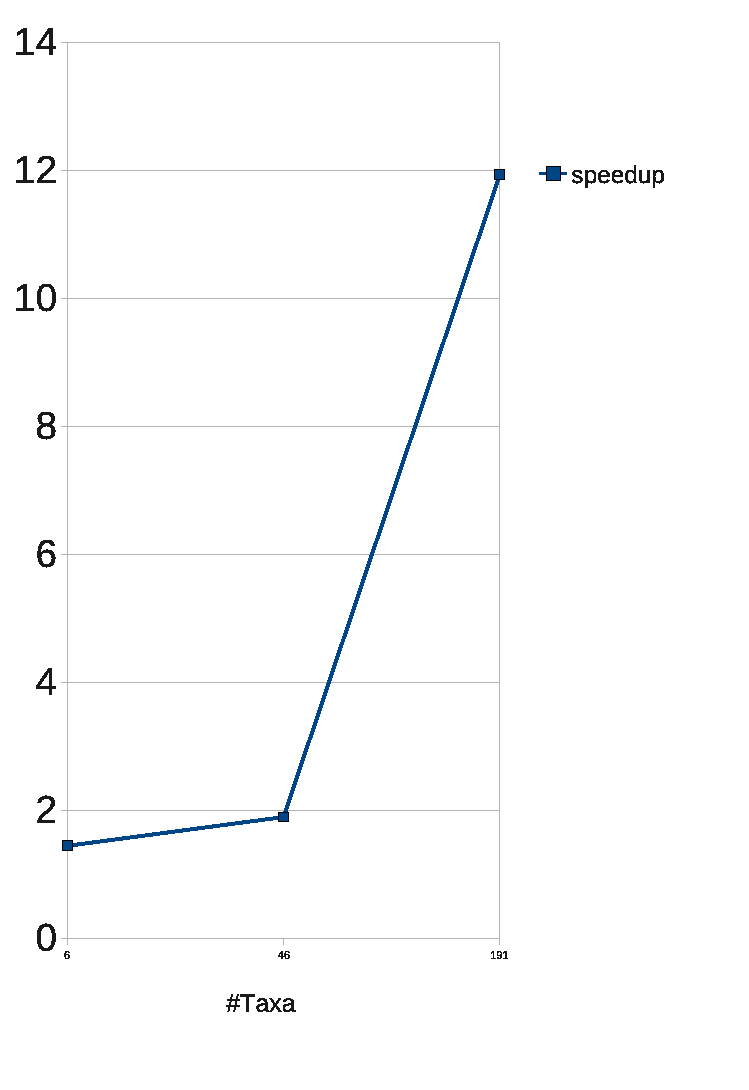
\includegraphics[width=\textwidth]{speedup.png}
\end{frame}


\section{Summary}
\begin{frame}{Summary Beast 2.0}

Extensibility
\begin{itemize}
\item Everything is a plug-in
\item Plug-in implementation:
\begin{itemize}
\item Add @Description annotation
\item Specify Inputs
\item Implement initAndValidate
\item Optional: getCitation, store, restore
\end{itemize}
\item Get xml-parsing, Input validation, xml-documentation for free
\item Store/restore more transparent
\item Explicit state object
\end{itemize}

Documentation
\begin{itemize}
\item Framework 'forces' proper documentation habits
\item Automatic documentation generation
\end{itemize}

Performance
\begin{itemize}
\item Up to 1 order of magnitude better performance
\end{itemize}
\end{frame}

\if0
\section{Other}
\begin{frame}{Mercator Projections}
\includegraphics[width=\textwidth]{mercator/mercator.png}
\end{frame}
\begin{frame}{Mercator Projections}
\includegraphics[width=\textwidth]{mercator/mercatornz.png}
\end{frame}
\begin{frame}{Mercator Projections}
\includegraphics[width=\textwidth]{mercator/mercatorla.png}
\end{frame}
\begin{frame}{Mercator Projections}
\includegraphics[width=\textwidth]{mercator/mercatoreur.png}
\end{frame}
\begin{frame}{Mercator Projections}
\includegraphics[width=\textwidth]{mercator/mercatorchin.png}
\end{frame}
\begin{frame}{Mercator Projections}
\includegraphics[width=\textwidth]{mercator/mercatornz.png}
\end{frame}
\begin{frame}{Mercator Projections}
\includegraphics[width=\textwidth]{mercator/mercatornz2.png}
\end{frame}
\begin{frame}{Mercator Projections}
\includegraphics[width=\textwidth]{mercator/mercatornz3.png}
\end{frame}
\fi
\end{document}



